\flushbottom

%%
%% Add problems.
%%




%%============================================================================
%%============================================================================
\chapter{Self-Adjoint Boundary Value Problems}



Seize the day and throttle it.

\begin{flushright}
  -Calvin\footnote{That's Calvin of ``Calvin and Hobbes'' of course.}
\end{flushright}







%%============================================================================
\section{Summary of Adjoint Operators}

The adjoint of the operator
\index{adjoint!of operators}
\[ 
L[y] = p_n \frac{\dd^n y}{\dd x^n} + p_{n-1} \frac{\dd^{n-1} y}{\dd x^{n-1}} + \cdots + p_0 y,
\]
is defined
\[ 
L^*[y] = (-1)^n \frac{\dd^n}{\dd x^n} (\overline{p_n} y) + (-1)^{n-1}
\frac{\dd^{n-1}}{\dd x^{n-1}}(\overline{p_{n-1}} y) + \cdots + \overline{p_0} y 
\]

If each of the $p_k$ is $k$ times continuously differentiable and $u$ and 
$v$ are $n$ times continuously differentiable on some interval, then on that
interval Lagrange's identity states
\index{Lagrange's identity}
\[ \overline{v}L[u] - u \overline{L^*[v]} = \frac{\dd}{\dd x} B[u,v] \]
where $B[u,v]$ is the bilinear form
\[ B[u,v] = \sum_{m=1}^n \ \sum_{\substack{ j+k=m-1 \\ j\geq 0, k \geq 0 }}
(-1)^j u^{(k)} (p_m \overline{v})^{(j)}.\]
If $L$ is a second order operator then
\[ \overline{v} L[u] - u \overline{L^*[v]} = u'' p_2 \overline{v} + u' p_1 \overline{v} 
+ u \big[-p_2 \overline{v}'' + (-2 p_2' + p_1)
\overline{v}' + (-p_2'' + p_1')\overline{v}\big]. \]

Integrating Lagrange's identity on its interval of validity
gives us Green's formula.
\index{Green's formula}
\[ \int_a^b \left( \overline{v} L[u] - u \overline{L^*[v]} \right)\,\dd x =
\langle v | L[u] \rangle - \langle L^*[v] | u\rangle = 
B[u,v] \big|_{x=b} - B[u,v] \big|_{x=a} \]















%%============================================================================
\section{Formally Self-Adjoint Operators}
\index{formally self-adjoint operators}


\begin{Example}
  \label{ex_sa}
  The linear operator
  \[ L[y] = x^2 y'' + 2 x y' + 3 y \]
  has the adjoint operator
  \begin{align*} 
    L^*[y] &= \frac{\dd^2}{\dd x^2} (x^2 y) - \frac{\dd}{\dd x} (2x y) + 3y \\
    &= x^2 y'' + 4 x y' + 2y - 2 x y' - 2y + 3y \\
    &= x^2 y'' + 2x y' + 3y.
  \end{align*}
\end{Example}



In Example~\ref{ex_sa}, the adjoint operator is the same as the operator. 
If $L = L^*$, the operator is said to be \textbf{formally self-adjoint}.








Most of the differential equations that we study in this book are 
second order, formally self-adjoint, with real-valued coefficient functions.
Thus we wish to find the general form of this operator.
Consider the operator
\[ L[y] = p_2 y'' + p_1 y' + p_0 y,\]
where the $p_j$'s are real-valued functions.
The adjoint operator then is
\begin{align*}
  L^*[y] &= \frac{\dd^2}{\dd x^2} (p_2 y) - \frac{\dd}{\dd x} (p_1 y) + p_0 y \\
  &= p_2 y'' + 2p_2' y' + p_2'' y - p_1 y' - p_1' y + p_0 y \\
  &= p_2 y'' + (2p_2' - p_1) y' + (p_2'' - p_1' + p_0) y.
\end{align*}

Equating $L$ and $L^*$ yields the two equations,
\begin{alignat*}{2}
  &2p_2' - p_1 = p_1, &\qquad &p_2'' - p_1' + p_0 = p_0 \\
  &p_2' = p_1, &\qquad &p_2'' = p_1'.
\end{alignat*}

Thus second order, formally self-adjoint operators with real-valued coefficient
functions have the form
\[ L[y] = p_2 y'' + p_2' y' + p_0 y,\]
which is equivalent to the form
\[ L[y] = \frac{\dd}{\dd x} (p y') + q y.\]


Any linear differential equation of the form
\[ L[y] = y'' + p_1 y' + p_0 y = f(x), \]
where each $p_j$ is $j$ times continuously differentiable and real-valued, 
can be written as a formally self adjoint equation.
We just multiply by the factor, 
\[
\e^{P(x)} = \exp(\int^x p_1(\xi)\,\dd \xi)
\]
to obtain
\begin{gather*}
  \exp\left[P(x) \right] (y'' + p_1 y' + p_0 y) =  
  \exp\left[ P(x) \right] f(x) \\
  \frac{\dd}{\dd x} \left( \exp\left[ P(x) \right] y' \right) + 
  \exp\left[ P(x) \right] p_0 y 
  = \exp\left[ P(x) \right]f(x) .
\end{gather*}




\begin{Example}
  Consider the equation
  \[ y'' + \frac{1}{x} y' + y = 0. \]
  Multiplying by the factor
  \[ \exp \left(\int^x \frac{1}{\xi}\,\dd \xi \right) = \e^{\log x} = x \]
  will make the equation formally self-adjoint.
  \begin{gather*}
    x y'' + y' + x y = 0 \\
    \frac{\dd}{\dd x} (x y') + x y = 0
  \end{gather*}
\end{Example}



\begin{Result}
  If $L = L^*$ then the linear operator $L$ is formally self-adjoint.  Second
  order formally self-adjoint operators have the form
  \[ L[y] = \frac{\dd}{\dd x}(p y') + q y.\]
  Any differential equation of the form
  \[ L[y] = y'' + p_1 y' + p_0 y = f(x), \]
  where each $p_j$ is $j$ times continuously differentiable and real-valued, 
  can be written as a formally self adjoint equation by multiplying the 
  equation by the factor $\exp(\int^x p_1(\xi)\,\dd \xi)$.
\end{Result}






%%============================================================================
\section{Self-Adjoint Problems}

Consider the $n^{t h}$ order formally self-adjoint equation $L[y] = 0$,
on the domain $a \leq x \leq b$ subject to the boundary conditions,
$B_j[y] = 0$ for $j = 1, \ldots, n$.
where the boundary conditions can be written
\[ B_j[y] = \sum_{k=1}^n \alpha_{j k} y^{(k-1)}(a) + \beta_{j k} y^{(k-1)}(b) = 0 .\]

If the boundary conditions are such that Green's formula reduces to
\[ \langle v | L[u] \rangle - \langle L[v]| u \rangle = 0\]
then the problem is \textbf{self-adjoint}



\begin{Example}
  Consider the formally self-adjoint equation $-y'' = 0$, subject to the boundary
  conditions $y(0) = y(\pi) = 0$.
  Green's formula is
  \begin{align*}
    \langle v | -u'' \rangle - \langle -v'' | u \rangle
    &= [u' (-\overline{v}) - u (- \overline{v})']_0^\pi \\
    &= [u\overline{v}' - u' \overline{v}]_0^\pi \\
    &= 0.
  \end{align*}
  Thus this problem is self-adjoint.
\end{Example}




















%%============================================================================
\section{Self-Adjoint Eigenvalue Problems}

Associated with the self-adjoint problem
\[ 
L[y] = 0, \quad \mathrm{subject to} \quad B_j[y] = 0,
\]
is the eigenvalue problem
\[ 
L[y] = \lambda y, \quad \mathrm{subject to} \quad B_j[y] = 0.
\]
This is called a self-adjoint eigenvalue problem. 
The values of $\lambda$ for which there exist nontrivial solutions to
this problem are called eigenvalues.  The functions that satisfy the equation
when $\lambda$ is an eigenvalue are called eigenfunctions.






\begin{Example}
  Consider the self-adjoint eigenvalue problem
  \[ 
  -y'' = \lambda y, \quad \mathrm{subject to} \quad y(0) = y(\pi) = 0.
  \]
  First consider the case $\lambda = 0$.  The general solution is
  \[ 
  y = c_1 + c_2 x.
  \]
  Only the trivial solution satisfies the boundary conditions. 
  $\lambda = 0$ is not an eigenvalue.
  Now consider $\lambda \neq 0$.  The general solution is
  \[ 
  y = c_1 \cos \left(\sqrt{\lambda} x \right) 
  + c_2 \sin \left(\sqrt{\lambda} x\right).
  \]
  The solution that satisfies the left boundary condition is
  \[
  y = c \sin \left( \sqrt{\lambda} x \right).
  \]
  For non-trivial solutions, we must have
  \[
  \sin \left( \sqrt{ \lambda } \pi \right) = 0,
  \]
  \[
  \lambda = n^2, \quad n \in \mathbb{N}.
  \]
  Thus the eigenvalues $\lambda_n$ and eigenfunctions $\phi_n$ are
  \[ 
  \boxed{
    \lambda_n = n^2, \qquad \phi_n = \sin(n x), \qquad 
    \mathrm{for}\ n = 1, 2, 3, \ldots 
    }
  \]
\end{Example}







Self-adjoint eigenvalue problems have a number a interesting properties.  We
will devote the rest of this section to developing some of these 
properties.


\paragraph{Real Eigenvalues.}  The eigenvalues of a self-adjoint problem
are real.  Let $\lambda$ be an eigenvalue with the eigenfunction $\phi$.
Green's formula states
\begin{gather*}
  \langle \phi | L[\phi] \rangle - \langle L[\phi] | \phi \rangle = 0 \\
  \langle \phi | \lambda \phi \rangle - \langle \lambda \phi | \phi \rangle = 0 \\
  (\lambda - \overline{\lambda}) \langle \phi | \phi \rangle = 0
\end{gather*}
Since $\phi \not\equiv 0$, $\langle \phi | \phi \rangle > 0$.  Thus 
$\lambda = \overline{\lambda}$ and $\lambda$ is real.







\paragraph{Orthogonal Eigenfunctions.}
The eigenfunctions corresponding to distinct eigenvalues are orthogonal. 
Let $\lambda_n$ and $\lambda_m$ be distinct eigenvalues with the
eigenfunctions $\phi_n$ and $\phi_m$.  Using Green's formula,
\begin{gather*}
  \langle \phi_n | L[\phi_m] \rangle - \langle L[\phi_n] | \phi_m \rangle = 0 \\
  \langle \phi_n | \lambda_m \phi_m \rangle - \langle \lambda_n \phi_n | \phi_m \rangle=0\\
  (\lambda_m - \overline{\lambda_n})\langle \phi_n | \phi_m \rangle = 0. \\
  \intertext{Since the eigenvalues are real,}
  (\lambda_m - \lambda_n) \langle \phi_n | \phi_m \rangle = 0 .
\end{gather*}
Since the two eigenvalues are distinct, $\langle \phi_n | \phi_m \rangle = 0$
and thus $\phi_n$ and $\phi_m$ are orthogonal.







\paragraph{*Enumerable Set of Eigenvalues.}
The eigenvalues of a self-adjoint eigenvalue problem form an enumerable
set with no finite cluster point.  Consider the problem
\[ L[y] = \lambda y\ \mathrm{on}\ a \leq x \leq b, 
\qquad \mathrm{subject to}\ B_j[y] = 0. \]
Let $\{ \psi_1, \psi_2, \ldots, \psi_n \}$ be a fundamental set of solutions
at $x = x_0$ for some $a \leq x_0 \leq b$.  That is,
\[ \psi_j^{(k-1)}(x_0) = \delta_{j k}.\]
The key to showing that the eigenvalues are enumerable, is that the
$\psi_j$ are entire functions of $\lambda$. That is, they are 
analytic functions of $\lambda$ for all finite $\lambda$.  We will 
not prove this.

The boundary conditions are
\[ B_j[y] = \sum_{k=1}^n \left[ \alpha_{j k} y^{(k-1)}(a) 
  + \beta_{j k}y^{(k-1)}(b)\right] = 0.\]
The eigenvalue problem has a solution for a given value of $\lambda$ if
$y = \sum_{k=1}^n c_k \psi_k$ satisfies the boundary conditions.  That is,
\[ B_j \left[ \sum_{k=1}^n c_k \psi_k \right] 
= \sum_{k=1}^n c_k B_j[\psi_k] = 0
\quad \mathrm{for}\ j = 1, \ldots, n.\]

Define an $n \times n$ matrix $M$ such that $M_{j k} = B_k[\psi_j]$. 
Then if $\vec{c} = (c_1, c_2, \ldots, c_n)$, the boundary conditions can 
be written in terms of the matrix equation $M \vec{c} = 0$.  This equation
has a solution if and only if the determinant of the matrix is zero.
Since the $\psi_j$ are entire functions of $\lambda$,
$\Delta[M]$ is an entire function of $\lambda$.  The eigenvalues are real,
so $\Delta[M]$ has only real roots.  Since $\Delta[M]$ is an entire
function, (that is not identically zero), with only real roots, the roots
of $\Delta[M]$ can only cluster at infinity.  Thus the eigenvalues of
a self-adjoint problem are enumerable and can only cluster at infinity.

An example of a function whose roots have a finite cluster point is
$\sin(1/x)$.  This function, (graphed in Figure~\ref{fin_clust}), is
clearly not analytic at the cluster point $x = 0$.



\begin{figure}[h!]
  \begin{center}
    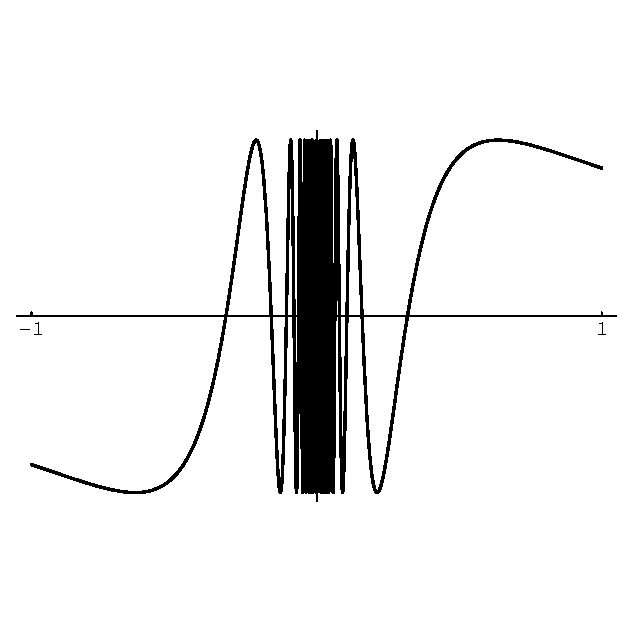
\includegraphics[width=0.6\textwidth]{ode/self_adjoint_bvp/finclust}
  \end{center}
  \caption{Function with a finite cluster point.}
  \label{fin_clust}
\end{figure}









\paragraph{Infinite Number of Eigenvalues.}
Though we will not show it, self-adjoint problems have an infinite number
of eigenvalues. Thus the eigenfunctions form an infinite orthogonal set.







\paragraph{Eigenvalues of Second Order Problems.}
Consider the second order, self-adjoint eigenvalue problem
\[ L[y] = (p y')' + q y = \lambda y, \quad \mathrm{on}\ a \leq x \leq b,
\quad \mathrm{subject to}\ B_j[y] = 0.\]
Let $\lambda_n$ be an eigenvalue with the eigenfunction $\phi_n$.
\begin{gather*}
  \langle \phi_n | L[\phi_n] \rangle = \langle \phi_n | \lambda_n \phi_n \rangle \\
  \langle \phi_n | (p \phi_n')' + q \phi_n \rangle = \lambda_n 
  \langle \phi_n | \phi_n \rangle \\
  \int_a^b \overline{\phi_n} (p \phi_n')'\,\dd x + \langle \phi_n | q | \phi_n\rangle
  = \lambda_n \langle \phi_n | \phi_n \rangle \\
  \big[\overline{\phi_n} p \phi_n'\big]_a^b - \int_a^b \overline{\phi_n}' p \phi_n'\,\dd x
  + \langle \phi_n | q | \phi_n\rangle = \lambda_n \langle \phi_n | \phi_n \rangle \\
  \boxed{ \lambda_n = \frac{[p \overline{\phi_n} \phi_n']_a^b 
      - \langle \phi_n' | p | \phi_n' \rangle + \langle \phi_n | q | \phi_n \rangle}
    { \langle \phi_n | \phi_n \rangle } }
\end{gather*}

Thus we can express each eigenvalue in terms of its eigenfunction.  You
might think that this formula is just a shade less than worthless.  When
solving an eigenvalue problem you have to find the eigenvalues before
you determine the eigenfunctions.  Thus this formula could not be used
to compute the eigenvalues.  However, we can often use the formula to
obtain information about the eigenvalues before we solve a problem.




\begin{Example}
  Consider the self-adjoint eigenvalue problem
  \[ -y'' = \lambda y, \qquad y(0) = y(\pi) = 0.\]
  The eigenvalues are given by the formula
  \begin{align*}
    \lambda_n &= \frac{\big[(-1) \overline{\phi} \phi'\big]_a^b 
      - \langle \phi_n' | (-1) | \phi_n'\rangle
      + \langle \phi_n | 0 | \phi_n \rangle }
    {\langle \phi_n | \phi_n \rangle} \\
    &= \frac{0 + \langle \phi_n' | \phi_n' \rangle + 0}{\langle \phi_n | \phi_n \rangle}.
  \end{align*}
  We see that $\lambda_n \geq 0$.  If $\lambda_n = 0$ then $\langle \phi_n' | \phi_n' \rangle
  = 0$,which implies that $\phi_n = \mathrm{const}$.  The only constant that
  satisfies the boundary conditions is $\phi_n = 0$ which is not an 
  eigenfunction since it is the trivial solution.  Thus the eigenvalues are 
  positive.
\end{Example}













%%============================================================================
\section{Inhomogeneous Equations}



Let the problem,
\[ 
L[y] = 0, \quad B_k[y] = 0,
\]
be self-adjoint.  If the inhomogeneous problem,
\[ 
L[y] = f, \quad B_k[y] = 0,
\]
has a solution, then we we can write this solution in terms of the 
eigenfunction of the associated eigenvalue problem,
\[ 
L[y] = \lambda y, \quad B_k[y] = 0.
\]


We denote the eigenvalues as $\lambda_n$ and the eigenfunctions as $\phi_n$ for 
$n \in \mathbb{Z}^+$.  For the moment we assume that $\lambda = 0$ is not an 
eigenvalue and that the eigenfunctions are real-valued.  We expand the 
function $f(x)$ in a series of the eigenfunctions.
\[
f(x) = \sum f_n \phi_n(x), \quad
f_n = \frac{ \langle \phi_n | f \rangle }{ \| \phi_n \| }
\]
We expand the inhomogeneous solution in a series of eigenfunctions and 
substitute it into the differential equation.
\begin{gather*}
  L[y] = f
  \\
  L \left[ \sum y_n \phi_n(x) \right] = \sum f_n \phi_n(x)
  \\
  \sum \lambda_n y_n \phi_n(x) = \sum f_n \phi_n(x)
  \\
  y_n = \frac{f_n}{\lambda_n}
\end{gather*}
The inhomogeneous solution is
\begin{equation}
  \label{y=sumfnflfnfnfn}
  y(x) = \sum \frac{ \langle \phi_n | f \rangle }{ \lambda_n \| \phi_n \| } \phi_n(x).
\end{equation}

As a special case we consider the Green function problem,
\[ 
L[G] = \delta(x - \xi), \quad B_k[G] = 0,
\]
We expand the Dirac delta function in an eigenfunction series.
\[
\delta(x - \xi) 
= \sum \frac{ \langle \phi_n | \delta \rangle }{ \| \phi_n \| } \phi_n(x)
= \sum \frac{ \phi_n(\xi) \phi_n(x) }{ \| \phi_n \| }
\]
The Green function is
\[
G(x|\xi) = \sum \frac{ \phi_n(\xi) \phi_n(x) }{ \lambda_n \| \phi_n \| }.
\]
We corroborate Equation~\ref{y=sumfnflfnfnfn} by solving the inhomogeneous 
equation in terms of the Green function.
\begin{gather*}
  y = \int_a^b G(x|\xi) f(\xi) \,\dd \xi
  \\
  y = \int_a^b \sum \frac{ \phi_n(\xi) \phi_n(x) }{ \lambda_n \| \phi_n \| } f(\xi) \,\dd \xi
  \\
  y = \sum \frac{ \int_a^b \phi_n(\xi) f(\xi) \,\dd \xi }{ \lambda_n \| \phi_n \| } \phi_n(x) 
  \\
  y = \sum \frac{ \langle \phi_n | f \rangle }{ \lambda_n \| \phi_n \| } \phi_n(x)
\end{gather*}











\begin{Example}
  Consider the Green function problem
  \[
  G'' + G = \delta(x - \xi), \quad G(0|\xi) = G(1|\xi) = 0.
  \]
  First we examine the associated eigenvalue problem.
  \begin{gather*}
    \phi'' + \phi = \lambda \phi, \quad \phi(0) = \phi(1) = 0
    \\
    \phi'' + (1 - \lambda)\phi = 0, \quad \phi(0) = \phi(1) = 0
    \\
    \lambda_n = 1 - (n \pi)^2, \quad \phi_n = \sin(n \pi x), \quad n \in \mathbb{Z}^+
  \end{gather*}
  We write the Green function as a series of the eigenfunctions.
  \[
  G(x|\xi) = 2 \sum_{n = 1}^\infty \frac{ \sin(n \pi \xi) \sin(n \pi x) }{ 1 - (n \pi)^2 }
  \]
\end{Example}










%% CONTINUE HERE
%% Do the \lambda = 0 case.





\raggedbottom
%%============================================================================
\exercises{
\pagebreak
\flushbottom
\section{Exercises}






%%-----------------------------------------------------------------------------
%%\begin{large}
%%\noindent
%%\textbf{}
%%\end{large}






%% L y = y^{(n)} + p_1(z) y^{(n-1)} + p_2(z) y^{(n-2)} + \cdots + p_n(z) y.
\begin{Exercise}
  \label{exercise adjoint operator n}
  Show that the operator adjoint to
  \[
  L y = y^{(n)} + p_1(z) y^{(n-1)} + p_2(z) y^{(n-2)} + \cdots + p_n(z) y
  \]
  is given by
  \[
  M y = (-1)^n u^{(n)} + (-1)^{n-1} (\overline{p_1(z)} u)^{(n-1)} 
  + (-1)^{n-2} (\overline{p_2(z)} u)^{(n-2)} + \cdots + \overline{p_n(z)} u.
  \]

  \hintsolution{adjoint operator n}
\end{Exercise}








\raggedbottom
}
%%============================================================================
\hints{
\pagebreak
\flushbottom
\section{Hints}




%%-----------------------------------------------------------------------------
%%\begin{large}
%%\noindent
%%\textbf{}
%%\end{large}




%% L y = y^{(n)} + p_1(z) y^{(n-1)} + p_2(z) y^{(n-2)} + \cdots + p_n(z) y.
\begin{Hint}
  \label{hint adjoint operator n}
  %% CONTINUE
\end{Hint}








\raggedbottom
}
%%============================================================================
\solutions{
\pagebreak
\flushbottom
\section{Solutions}






%%-----------------------------------------------------------------------------
%%\begin{large}
%%\noindent
%%\textbf{}
%%\end{large}







%% L y = y^{(n)} + p_1(z) y^{(n-1)} + p_2(z) y^{(n-2)} + \cdots + p_n(z) y.
\begin{Solution}
  \label{solution adjoint operator n}
  Consider $u(x), v(x) \in C^n$. ($C^n$ is the set of $n$ times continuously
  differentiable functions). First we prove the preliminary result
  \begin{equation}
    \label{eqn_uvn_unv}
    u v^{(n)} - (-1)^n u^{(n)} v = 
    \frac{\dd}{\dd x} \sum_{k=0}^{n-1} (-1)^k u^{(k)} v^{(n-k-1)}
  \end{equation}
  by simplifying the right side.
  \begin{align*}
    \frac{\dd}{\dd x} \sum_{k=0}^{n-1} (-1)^k u^{(k)} v^{(n-k-1)}
    &= \sum_{k=0}^{n-1} (-1)^k \left( u^{(k)} v^{(n-k)} 
      + u^{(k+1)} v^{(n-k-1)} \right) \\
    &= \sum_{k=0}^{n-1} (-1)^k u^{(k)} v^{(n-k)} 
    - \sum_{k=0}^{n-1} (-1)^{k+1} u^{(k+1)} v^{(n-k-1)} \\
    &= \sum_{k=0}^{n-1} (-1)^k u^{(k)} v^{(n-k)} 
    - \sum_{k=1}^{n} (-1)^{k} u^{(k)} v^{(n-k)} \\
    &= (-1)^0 u^{(0)} v^{n-0} - (-1)^n u^{(n)} v^{(n-n)} \\
    &= u v^{(n)} - (-1)^n u^{(n)} v
  \end{align*}

  We define $p_0(x) = 1$ so that we can write the operators in a nice form.
  \[
  L y = \sum_{m=0}^n p_m(z) y^{(n-m)}, \quad
  M u = \sum_{m=0}^n (-1)^m (\overline{p_m(z)} u)^{(n-m)}
  \]
  Now we show that $M$ is the adjoint to $L$.
  \begin{align*}
    \overline{u} L y - y \overline{M u}
    &= \overline{u} \sum_{m=0}^n p_m(z) y^{(n-m)}
    - y \sum_{m=0}^n (-1)^m (p_m(z) \overline{u})^{(n-m)} \\
    &= \sum_{m=0}^n \left( \overline{u} p_m(z) y^{(n-m)} 
      - (p_m(z) \overline{u})^{(n-m)} y 
    \right) \\
    \intertext{We use Equation~\ref{eqn_uvn_unv}.}
    &= \sum_{m=0}^n \frac{\dd}{\dd z} \sum_{k=0}^{n-m-1} 
    (-1)^k (\overline{u} p_m(z))^{(k)} y^{(n-m-k-1)}
  \end{align*}
  \[
  \boxed{
    \overline{u} L y - y \overline{M u} = \frac{\dd}{\dd z} \sum_{m=0}^n \sum_{k=0}^{n-m-1} 
    (-1)^k (\overline{u} p_m(z))^{(k)} y^{(n-m-k-1)}
    }
  \]
\end{Solution}








\raggedbottom
}
